\documentclass[11pt,a4paper,spanish]{book}

\usepackage[spanish]{babel}

\usepackage[utf8]{inputenc}

\usepackage{graphicx}

\usepackage[a4paper,left=3cm,right=2cm,top=3cm,bottom=2cm]{geometry}

\usepackage{url}

\title{Implementación paralela de un sistema de visión global por computadora}

\author{Cañibano, Rodrigo S.\and Grosclaude, Eduardo \and Balladini, Javier}

\begin{document}

\maketitle

\chapter{Introducción}

% vim: set spell spelllang=es syntax=tex :

\section{Fútbol de robots}

La \emph{RoboCup}\cite{robocupHist} (del inglés \emph{Robot World Cup}) es una
competencia internacional celebrada desde 1997, donde equipos de robots juegan
una versión simplificada del fútbol. Su finalidad es la de ofrecer un ambiente
controlado donde poner a prueba los avances en distintas áreas de conocimiento
como la inteligencia artificial, visión por computadora y robótica. Existen
cinco ligas distintas cuyas características varían desde la simulación del
ambiente y de los robots, hasta robots humanoides con visión local. De éstas, la
más antigua es la liga de tamaño pequeño (\emph{SSL}, del inglés \emph{Small
Size League}).

Nota de OSO: Se puede agregar info detallada de cada una de las ligas

Un partido de la \emph{SSL} enfrenta a dos equipos de seis robots, que deben
tener un tamaño menor que un cilindro de 9$cm$ de radio y 15$cm$ de
alto\cite{sslrules2015}. Los robots tienen capacidad de procesamiento reducida,
y cada equipo cuenta con una computadora fuera del campo de juego, a la cual se
delega la toma de decisiones. Estas computadoras perciben el ambiente a través
de un sistema de visión global centralizado compartido. Se utiliza un conjunto
de cámaras, montadas sobre distintas áreas del campo de juego y conectadas a una
computadora donde se ejecuta el sistema de visión. El sistema detecta la
posición y orientación de cada uno de los robots y la posición de la pelota, y
reporta esta información a las computadoras que controlan los equipos.

Para que el sistema de visión pueda identificar a cada robot, cada uno tiene
sobre su parte superior cinco parches de colores (Fig. \ref{sistemaVG}). El
parche que se encuentra en el centro indica el color del equipo del robot, y los
cuatro restantes sirven para identificar al robot dentro del equipo y para
conocer la orientación que lleva en cada momento. La pelota es de un color
uniforme y distinto al de los parches de los robots; normalmente, naranja, ya
que este color contrasta fácilmente con el verde de la cancha.

\begin{figure}[!h]

	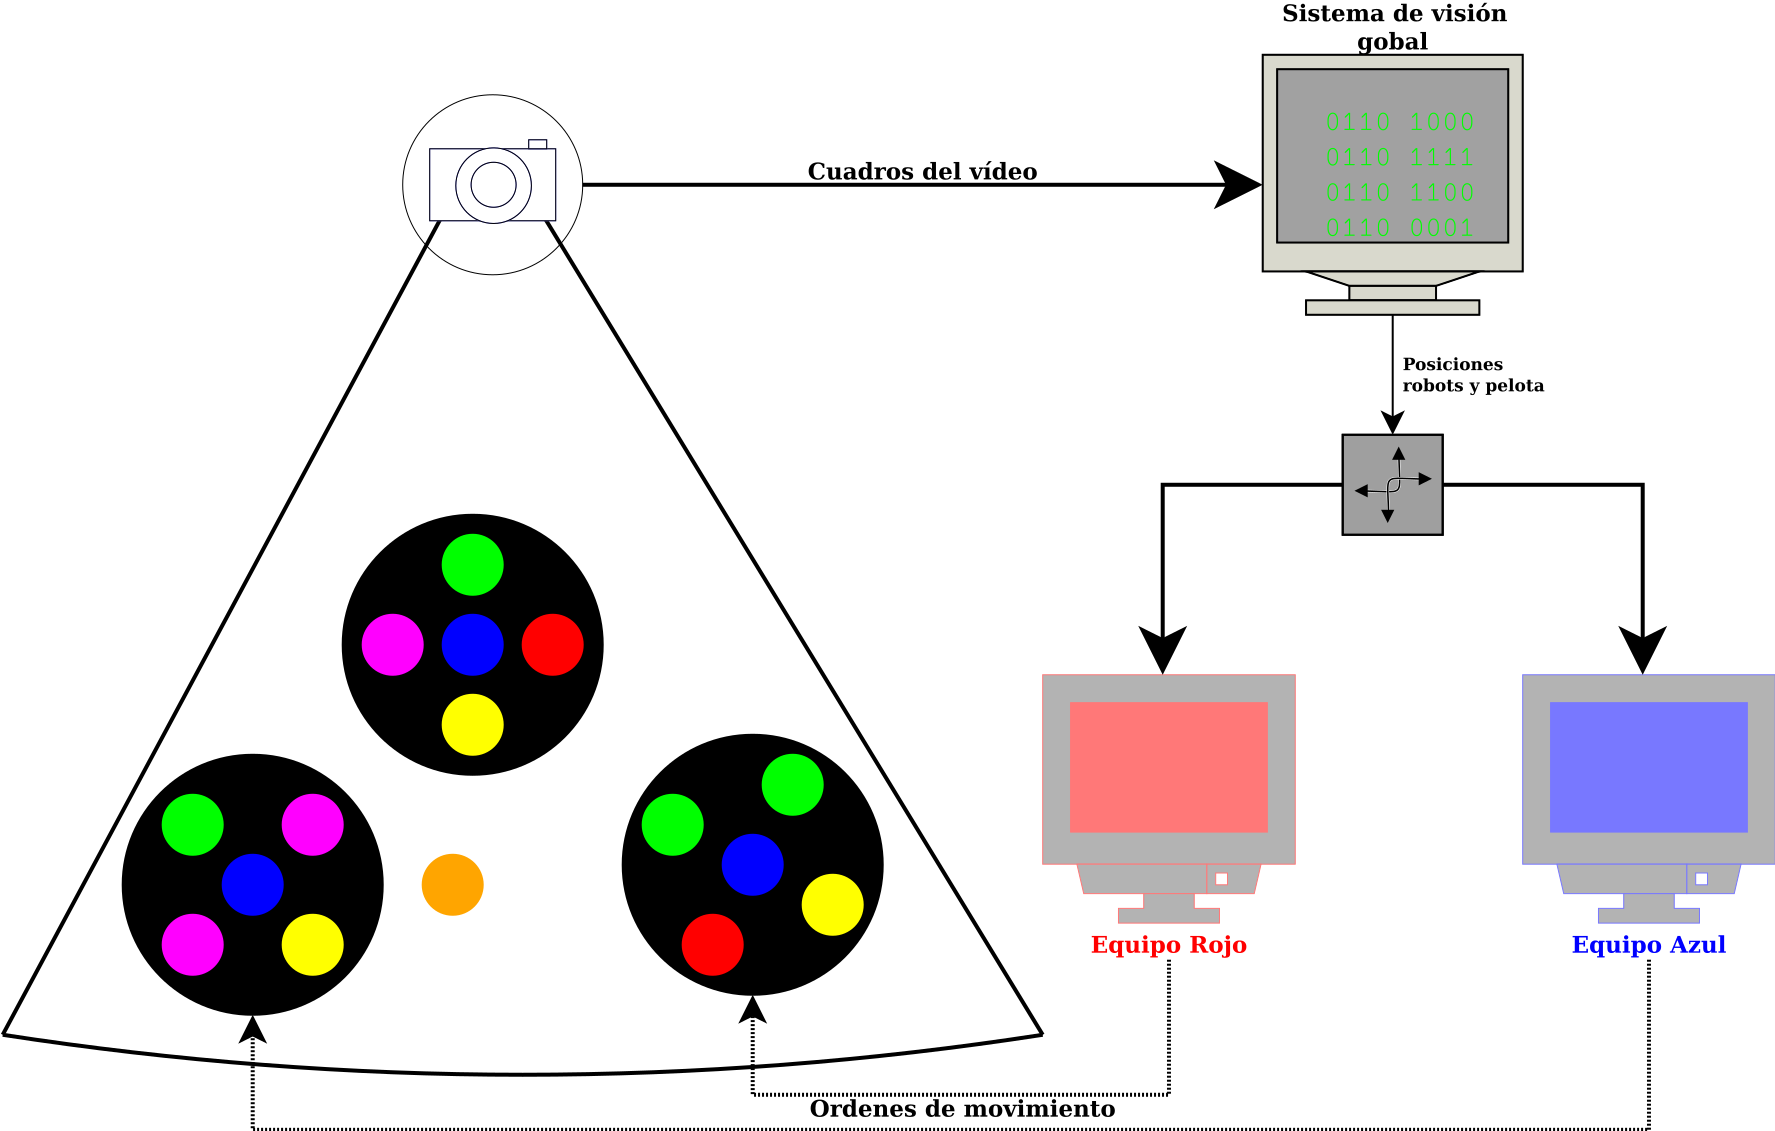
\includegraphics[width=\textwidth]{img/sistemaVG.pdf}

	\caption{Estructura de comunicación del sistema de visión global en
	fútbol de robots de la \emph{SSL}.}

	\label{sistemaVG}

\end{figure}

El uso de este sistema centralizado permite a los participantes abstraerse de
los problemas de la visión por computadora y enfocarse en la estrategia del
juego. Además, permite que las tareas de calibración y montaje de las cámaras se
realicen una sola vez para cada campo de juego, en vez de para cada partido.

Originalmente el tamaño de la cancha era de 4,9$m\times$3,4$m$, lo que permitía
que todo el campo de juego fuera observado con una sola cámara. Luego se optó
por dos tipos de canchas en los partidos de la \emph{SSL}: las canchas de tamaño
simple, con un tamaño de 6,05$m\times$4,05$m$ para las cuales se utilizan dos
cámaras, una sobre cada media cancha, y las de tamaño doble, con un tamaño de
8,09$m\times$6,05$m$, que utilizan cuatro cámaras, una por cada mitad de cada
media cancha (Fig. \ref{FALTA}). Desde el año 2015, las canchas de tamaño doble
son las utilizadas de forma predeterminada\cite{sslrules2015}. Con este cambio
se espera permitir la exploración de nuevas tácticas por parte de los equipos,
ya que una mayor área de juego permite a los robots movimientos de mayor
amplitud y variedad.

\begin{figure}[!h]

	\includegraphics[width=\textwidth]{img/FALTA.png}

	\caption{Dimensiones y área de cobertura de las cámaras en la liga
	\emph{SSL}, en competencias a) anteriores a 2015; b) año 2015 y
	posteriores.}

	\label{FALTA}

\end{figure}

Sin embargo, como consecuencia, en las canchas de tamaño doble, el sistema de
visión debe procesar cuatro veces más información que en las canchas originales;
lo que da lugar a un problema. En efecto, el fútbol de robots se desarrolla en
un contexto de tiempo real, ya que el ciclo completo de procesamiento de
información debe cumplirse en un plazo máximo para poder alcanzar los objetivos.
El servidor debe procesar cada cuadro para entregar la información de posición y
velocidad de cada elemento en el campo de juego a las computadoras coordinadoras
de los equipos; y éstas deben tomar una decisión y comunicarla a los robots,
todo dentro de un tiempo de respuesta razonable para el progreso de la
aplicación.

Los parámetros de calidad de este tipo de sistema son, normalmente:

\begin{itemize}

	\item 	tasa de aciertos en la detección de objetos;

	\item 	precisión en la posición y orientación de los aciertos en la
		detección de objetos;

	\item 	precisión en la posición y orientación de los robots y pelota;

	\item 	cuadros por segundo (\emph{FPS}, del inglés \emph{Frames Per
		Second}) procesados;

	\item 	y máximo tiempo de espera del cuadro (tiempo desde la creación
		del cuadro hasta la entrega de la información extraída).

\end{itemize}

Duplicar la cantidad de información que se debe procesar impacta negativamente
en el rendimiento de estos sistemas, debido a que se reducen los cuadros por
segundo procesados y se incrementa el tiempo de espera del cuadro. Para aumentar
el rendimiento de estos sistemas es necesario implementar soluciones paralelas
que aprovechen las múltiples unidades de procesamiento de las arquitecturas de
cómputo actuales.


% vim: set spell spelllang=es syntax=tex :

\section{Sistemas existentes de visión global para fútbol de robots físicos}


El software de visión global utilizado en la \emph{SSL} de la \emph{Robocup} es
el \emph{SSL-Vision}\cite{sslvision}. Este es un sistema programado en
\emph{C++} basado en plugins, lo que le permite ser extendido fácilmente
mediante estos. Lamentablemente, posee algunas desventajas en relación a la
escalabilidad y al uso educativo. En primer lugar, el sistema de captura de
cuadros y el de procesamiento están fuertemente acoplados formando parte del
mismo hilo de ejecución. Esto impide hacer uso de las capacidades de
paralelización que ofrece el hardware actual, limitando su desempeño y
escalabilidad. Para aumentar la eficiencia del sistema los plugins están
altamente optimizados aumentando la complejidad del sistema. Esta complejidad
entorpece su uso como herramienta didáctica para la introducción a la visión por
computadora.

En \cite{torres2014} se presenta un sistema destinado al uso educativo, basado
en pilas de plugins, y también programado en \emph{C++}. El framework tiene dos
hilos de búsqueda de objetos, uno para encontrar la pelota y otro para encontrar
los robots, un hilo de captura de cuadros de vídeo (desde un vídeo pre grabado o
una captura desde una cámara), y un hilo para la interfaz de usuario. Su grado
de paralelismo es mejor que el de \emph{SSL-Vision} pero aún así no permite
escalar a más de cuatro núcleos.

Bajo las condiciones para las que fue pensado este framework, el
desaprovechamiento de los recursos de hardware no es un problema, ya que el
sistema puede procesar un vídeo de 352x228 píxeles a una taza de 60 cuadros por
segundo. Sin embargo, actualmente se utiliza como fuente cuatro cámaras, en
lugar de la cámara única para la cual el sistema fue pensado. Cuando se probó el
framework con un vídeo con una resolución de 800x600 píxeles el número de
cuadros por segundos procesados cayo a 45 cuadros por segundo.


% vim: set spell spelllang=es syntax=tex :

\section{Objetivos}

\label{objetivos}

El objetivo de esta tesis es crear un sistema de visión global por computadora
para fútbol de robots de la \emph{SSL}, que pueda ser utilizado como herramienta
didáctica para la introducción a la visión por computadora y programación
paralela, y permita explorar distintas estrategias de paralelización sobre
máquinas de memoria compartida. El sistema debe ser escalable para soportar
todos los núcleos de procesamiento de las CPUs de cualquier máquina de memoria
compartida.

El sistema no hará uso de placas aceleradoras gráficas ni sistemas de memoria
distribuida por dos razones. Limitarse al uso de CPUs en sistemas de memoria
compartida permite su uso en cualquier computadora de escritorio o portátil,
facilitando la disponibilidad de equipos y permitiendo a los alumnos
experimentar en sus propias computadoras.


% vim: set spell spelllang=es syntax=tex :

\section{Metodología}

La presente tesis es del tipo experimental. Durante su realización se desarrolló
un nuevo sistema de visión global por computadora para fútbol de robots, basado
en plugins, paralelo, capaz de aprovechar hardware multi-core, sin limitaciones
arquitectónicas respecto de la cantidad de núcleos utilizables.

Para la construcción del nuevo sistema se tomó como base el sistema descripto en
\cite{torres2014}. Éste es un sistema basado en plugins, orientado al uso
educativo. Del mismo se utilizaron los plugins desarrollados en dicho trabajo,
modificándolos para que se integren al nuevo framework.

Para poder medir el rendimiento del nuevo sistema se consideraron dos variables.

\begin {itemize}

	\item	La primera variable es la cantidad de cuadros por segundo (o
		FPS, de sus siglas en inglés \emph{Frames per second})
		procesados por el sistema. Una tasa de cuadros por segundo más
		alta se considera beneficiosa, ya que significa que se provee a
		los equipos con más información cada segundo.

	\item	La segunda es el tiempo de espera máximo de los cuadros.
		Mientras menor sea el tiempo de espera del cuadro, la
		información entregada por el sistema será más actual, y por lo
		tanto más relevante.

\end {itemize}

Nota OSO: Acá no va algo de OpenMP? Y la forma de prueba?


% vim: set spell spelllang=es syntax=tex :

\section{Organización del trabajo}

Este trabajo de tesis fue estructurado en seis capítulos. En el capítulo
\ref{marcoTeorico} se presenta el marco teórico necesario para este trabajo. La
sección \ref{mt_visionComputadora} es una introducción a la visión por
computadora y las etapas que suelen definirse en un sistema de visión por
computadora. En la sección \ref{descripcionSistemaBase} se detalla el sistema de
visión global utilizado como base para el desarrollo del sistema propuesto en
este trabajo.  En la sección \ref{mt_modelosparalelos} se describen dos
clasificaciones que permiten distinguir los modelos computacionales de los
sistemas de cómputo paralelos. A continuación, en la sección \ref{mt_openmp} se
hace una introducción a \emph{OpenMP} y se explican sus modelos de computación y
las directivas utilizadas por el sistema propuesto.

En el capítulo \ref{sistemaPropuesto} se describe el sistema propuesto. La
sección \ref{descripcionSistema} describe las tareas del sistema y la forma en
la cual se fragmentan los datos. Luego, en la sección
\ref{implementacionFramework}, se describe la implementación.

En el capítulo \ref{experimentacion} se describen los experimentos realizados
utilizando el sistema desarrollado. Se comienza explicando la metodología
experimental en la sección \ref{metodologiaExperimental}, la plataforma
experimental se detalla en la sección \ref{plataformaExperimental}, y los
detalles de los experimentos y sus resultados son discutidos en la sección
\ref{resultados}.

En el capítulo \ref{usoEducativo} se plantean posibles usos del sistema como
herramienta didáctica para materias de sistemas paralelos, en la sección
\ref{eduparalelos}, y visión por computadora, en la sección \ref{eduvision}.

Finalmente en el capítulo \ref{conclucionesYTrabajosFuturos} se presentan las
conclusiones del trabajo, en la sección \ref{concluciones}, y los posibles
trabajos futuros, en la sección \ref{trabajosFuturos}.


\chapter{Marco teórico}

% vim: set spell spelllang=es syntax=tex :

\section{Visión por computadora}

La visión por computadora es una disciplina cuyo objetivo principal es definir
un modelo de una escena a partir de imágenes\cite{cvLinda2001}. Como
consecuencia se estudian los métodos captura y procesamiento.

Agregar
https://en.wikipedia.org/wiki/Computer_vision#Computer_vision_system_methods

y digitalImageProcessing2ed.


% vim: set spell spelllang=es syntax=tex :

\section{Descripción del sistema de visión global para fútbol de robots
físicos sobre el que se basa la presente propuesta}
\sectionmark{Descripción del sistema de visión global para fútbol de robots
físicos...}

El sistema descripto en \cite{torres2014} tiene como objetivo ser utilizado como
herramienta didáctica para la introducción a la visión por computadora. Éste
sistema esta basado en pilas de plugins y desacopla el hilo de captura del los
hilos de búsqueda. Se utilizan múltiples hilos para aprovechar hasta cuatro
núcleos (para el fútbol de robots), pero si el sistema pose mas núcleos estos no
son utilizados. El sistema define un framework de visión por computadora capas
de adaptarse a distintos dominios, pero se provee una solución especifica para
el fútbol de robots de tamaño pequeño. El framework general tiene tres
componentes principales:

\begin{description}

	\item[Hilo principal:] es el hilo encargado de la interfaz gráfica de
		usuario.
	
	\item[Hilo de captura de cuadros:] es el hilo encargado de la captura o
		generación de los cuadros a partir de una cámara o archivo.

	\item[Hilos de procesamiento de cuadros:] estos hilos están formados por
		una pila de plugins que procesaran cada cuadro en forma
		secuencial. Normalmente, por cada tipo de objeto a reconocer,
		hay un hilo de este tipo dedicado a su detección. La diferencia
		entre cada uno de ellos esta en los plugins que componen la pila
		y en su orden. Existen mecanismos de control para asegurar que
		si un cuadro es procesado por hilo de procesamiento entonces
		sera procesado por el resto de los hilos de procesamiento,
		mientras que al mismo tiempo se asegura que cada cuadro se
		procese solo una ves por cada hilo.

\end{description}

En la implementación de la solución especifica para el fútbol de robots de la
\emph{SSL}, se crean dos hilos de
procesamiento de cuadros, uno para la búsqueda de los robots y la otro para la
búsqueda de la pelota. Las primeras etapas de procesamiento son iguales en
ambos. Los primeros plugins son los de conversión de color, segmentación de
color y morfología. El hilo de procesamiento que busca la pelota continua con el
plugin de búsqueda de pelota, mientras que aquel encargado de la búsqueda de
robots continua con los plugins de detección de regiones principales y detección
de detecciones secundarias. Ambos terminan con el plugin de difusión. De
acuerdo a su función, los plugins pueden ser agrupados por las etapas de la
visión por computadora que implementan:

\begin{description}

\item[Adquisicion de la imagen:] Esta etapa esta a cargo del hilo de captura de
	cuadros.

\item[Pre procesamiento:] plugins de conversión de color, de segmentación de
	color y de morfología.

\item[Extraccion de características, Detección y Segmentación:] plugins de
	detección de regiones principales.

\item[Procesamiento de alto nivel:] plugins de detección de pelota y de
	detección de regiones secundarias.

\item[Toma de decisiones:] Dado que el sistema de visión para fútbol de robots
	no realiza toma de decisiones, el estado de la cancha es comunicado a
	las computadoras de los equipos a través del plugin de difusión.

\end{description}

La generación de los cuadros y su procesamiento son independientes, y los
tiempos de generación y procesamiento pueden ser distintos y variables, por lo
cual es necesario un buffer entre el hilo de captura de cuadros y los hilos de
procesamiento de cuadros. En caso de que el buffer alcance su capacidad máxima,
se descartan los cuadros mas viejos.


\chapter{Framework propuesto}

% vim: set spell spelllang=es syntax=tex :

\section{Descripción del framework}

Para aumentar el throughput del sistema se aplicaran las dos técnicas discutidas
con anterioridad. En primer lugar el sistema no estará limitado a tomar solo un
cuadro por ves. La segunda optimización consta en dividir cada cuadro para que
cada parte pueda ser procesada por un thread distinto. También debe mantenerse
que las distintas pilas de plugins ejecuten de forma independiente una de la
otra.

Para esto se propone la siguiente secuencia de procesamiento para cada ítem (un
cuadro en el caso de la solución especifica para fútbol de robots):

\begin{enumerate}

\setcounter{enumi}{-1}

\item	Antes de la ejecución el usuario establece una cantidad máxima de tareas
	en ejecución simultanea.

\item	El hilo de captura genera o captura un ítem y lo deposita en el buffer.

\item	Una tarea maestra consume el ítem mas reciente del buffer y crea una
	tarea de búsqueda para su procesamiento. Si hay mas tareas que las
	permitidas o no hay ítems en el buffer, espera.

\item	Cada tarea de búsqueda crea tantas tareas por cada una de sus pilas de
	\emph{plugins}. Mientras espera a que estas taras terminen no debe ser
	contada para el limite de tareas en ejecución.

\item	Cada tarea fracciona el ítem y crea tantas tareas como fragmentos del
	ítem se hallan creado. Esta tarea terminara tan pronto como sus tareas
	hijas terminen. Mientras espera no contribuirá al limite de tareas en
	ejecución.

\item	Las tareas procesaran cada fragmento utilizando la pila de
	\emph{plugins}. Antes de terminar eliminara el fragmento del ítem.

\item	Cuando terminan todas las tareas de las pilas de plugins, la tarea de
	búsqueda resume la ejecución para eliminar el ítem de la memoria y
	posiblemente realizar tareas conteo.

\end{enumerate}

Algo que no queda especificado en la descripción anterior, es la naturaleza de
las tareas. Por un lado, las tareas pueden comenzar su ejecución al momento de
ser creadas o pueden esperar a que la cantidad de tareas en ejecución sea menor
que el máximo establecido. La primera opción tiene como desventaja que dado que
el único control sobre la cantidad de tareas se realiza al consumir un ítem, la
cantidad de tareas en ejecución sea mayor al máximo establecido durante una
porción significativa de la duración del programa. La segunda opción solo
funcionara satisfactoriamente si se asegura que la próxima tarea a ejecutar sea
la mas antigua.

El establecer un máximo de hilos en ejecución nos permite asegurarnos de que los
hilos no compitan por la CPU y que esta se mantenga ocupada siempre que haya
tareas a realizar, simplemente estableciendo tal máximo como el números de
procesadores disponibles. Es por esto que la segunda opción es la mas deseable.

Las clases del framework básico son las siguientes:

\begin{description}

\item[Item]: Esta clase define un tipo genérico de los ítems que serán tratados
	por el sistema.

\item[RingBuffer]: Este es el buffer donde se guardan los ítems generados
	mientras esperan ser procesados. El buffer guarda solo punteros a
	objetos de la clase \emph{Item} y no tiene mecanismos de control que
	permitan acceder la estructura desde múltiples threads al mismo tiempo.
	Cuando se solicita un ítem, se devuelve el puntero al mas recientemente
	agregado o \textbf{NULL} en caso de que la estructura este vacía. Cuando
	se intenta agregar un nuevo ítem pero la estructura esta llena se coloca
	este en lugar del ítem mas viejo en la estructura y se retorna el
	puntero a este al llamador, delegándole su destrucción. La destrucción
	del ítem se delega al llamador por dos motivos. El primero es que el
	buffer desconoce el tipo real del ítem. La segunda razón es que para
	poder ser utilizado de forma segura, las llamadas a los métodos del
	buffer deben estar dentro de secciones criticas y realizar las
	eliminaciones dentro de estas podría ser muy lento.

\item[Input]: Se trata de una clase que funciona como definición de la interfaz
	de las clases que generan los ítems. Sus métodos principales son
	\emph{run} y \emph{generate}. El método \emph{generate} debe ser re
	implementado por las clases hijas para generar el tipo de ítem
	especifico del sistema. El método \emph{run} es el encargado de generar
	los ítems llamando a \emph{generate} y colocarlos en el
	\emph{RingBuffer}. Este último método puede ser redefinido si la
	aplicación así lo requiere.

\item[ItemSlicer]: Es la clase que define la interfaz de las clases encargadas
	de dividir los ítems. Se definen dos métodos. El primero es \emph{slice}
	que recibe como parámetro ítem y la cantidad de partes en la que este
	debe ser dividido y retorna un arreglo de ítems. El segundo método es
	\emph{delPart} que recibe como parámetro una de las partes creadas por
	el método \emph{slice} y la elimina.

\item[Plugin]: Esta clase define una interfaz para los plugins que realizaran
	las distintas partes del procesamiento de la imagen. Solo se define el
	método \emph{process} que tiene como único parámetro un puntero a un
	objeto de la clase \emph{Item}.

\item[PluginStack]: Esta es la clase que tomara el ítem y se encarga de
	entregarlo a cada uno de los plugins. Tiene solo dos métodos,
	\emph{addPlugin}, para agregar un plugin, y \emph{process} que tiene
	como parámetro un ítem, para procesar un ítem.

\item[ItemSwitch]: Es la clase encargada de tomar los cuadros del buffer, crear
	la partición utilizando la clase descendiente de \emph{ItemSlicer},
	crear las tareas para que las partes sean procesadas por las pilas de
	plugins y crear los hilos que ejecutaran las tareas. La cantidad hilos y
	la cantidad de partes en las cuales dividirá el ítem se definirán
	durante su creación.

\end{description}

\begin{figure}[h]

	\includegraphics[width=\textwidth]{img/clasesFramework.pdf}

	\caption{Diagrama de clases Framework base.}

\end{figure}

Para adaptar el framework para utilizarlo como un sistema de visión por
computadora para el fútbol de robots se incorporaron las siguientes clases, las
cuales fueron tomadas y modificadas del sistema de visión presentado en
\cite{torres2014}:


\begin{description}

\item[Frame]: Subclase de \emph{Item}. Contiene una imagen que representa un
	cuadro y una estructura auxiliar que contiene la información necesaria
	para el funcionamiento de los plugins.

\item[CaptureFromFile]: Subclase de \emph{Input}. Es la clase encargada de crear
	el flujo de objetos \emph{Frame}, tomando cada cuadro desde un archivo
	de vídeo.

\item[FrameSlicer]: Subclase de \emph{ItemSlicer}. En este caso lo que se divide
	es la imagen del cuadro. Cada sub cuadro tendrá un solapamiento con los
	adyacente ya que se debe evitar que un robots o la pelota no este
	totalmente contenido dentro de por lo menos un sub cuadro. Para
	minimizar el área solapada las particiones se realizan de manera tal que
	se minimice el perímetro pero ocupen la mayor área posible. Para lograr
	esto se busca la partición que haga que la relación entre el alto y el
	ancho sea lo mas cercana a uno.

\item[Subclases de \emph{Plugin}]: \emph{PluginBlur},
	\emph{PluginColorConversions}, \emph{PluginColorSegmentation},
	\emph{PluginDetectBalls}, \emph{PluginFindBlobs},
	\emph{PluginFindSecondariesBlobs}, \emph{PluginMorphology} y
	\emph{PluginNetworking}.

\item[Clases auxiliares]: \emph{ball}, \emph{colorspace}, \emph{datastruct},
	\emph{homography}, \emph{marker}, \emph{pattern},
	\emph{pattern\_matching}, \emph{practicalsocket}, \emph{segmentation},
	\emph{team}, \emph{timer}.

\end{description}

\begin{figure}[h]

	\includegraphics[width=\textwidth]{img/clasesFrameworkRobots.pdf}

	\caption{Diagrama de clases Framework del framework instanciado para el
	sistema de visión para el fútbol de robots.}

\end{figure}

Existen dos parámetros ajustables. El primero es la cantidad de hilos que
ejecutaran las tareas de búsqueda. El segundo parámetro es la cantidad de partes
en las cuales se dividirá el cuadro.


\chapter{Experimentación}

% vim: set spell spelllang=es syntax=tex :

\section{Resultados}

Para comprobar el funcionamiento del nuevo framework se utilizaron los vídeos de
resolución 640x480, 800x600 y 1280x720, en el equipo con procesador Intel Xeon
E5-2630 con 16GiB de memoria ram.

Se realizaron pruebas con cada vídeo, variando la cantidad de partes en las que
fueron divididos los cuadros y la cantidad de cuadros procesados al mismo tiempo
entre uno y doce. Se ejecuto el programa durante 10 segundos. Se contó la
cantidad de cuadros procesados en ese tiempo y el retardo máximo la creación de
un cuadro y la finalización de su procesamiento. Cable aclarar que estas
estadísticas tienen solo en cuenta el procesamiento de los cuadros, no si se
encontraron los robots o pelota en ellos. Los resultados finales pueden verse
en las siguientes tablas.

//tablas de tiempo y retardo.

//Poner gráfico de retardo/cuadros


\bibliographystyle{plain}

\bibliography{biblio}

\end{document}
